\section{An\'alisis 2: Universidad de Sydney}
Vamos a realizar un an\'alisis de nuestro traceroute sobre la universidad de la capital australiana.\newline

El host de dicha universidad es http://sydney.edu.au/ (IP: 129.78.5.8).\\	

Página web de geolocalización de IP utilizada: \url{http://www.geoiptool.com/es/}.\\

Proveedor de Internet: Fibertel.

\subsubsection{Par\'ametros de entrada}
\begin{itemize}
\item Host: sydney.edu.au
\item Tiempo Limite: 5
\item Cant. Iteraciones en cada nodo: 10
\item Recorrido m\'aximo de nodos: 30 (TTL m\'aximo)
\item alpha: 0.05
\end{itemize}
El tiempo limite indica cuanto esperar de respuesta, como m\'aximo, a un nodo.\newline

\subsubsection{Resultados obtenidos}

Captura general de los resultados obtenidos: \newline


\begin{figure}[h]
	\begin{center}
    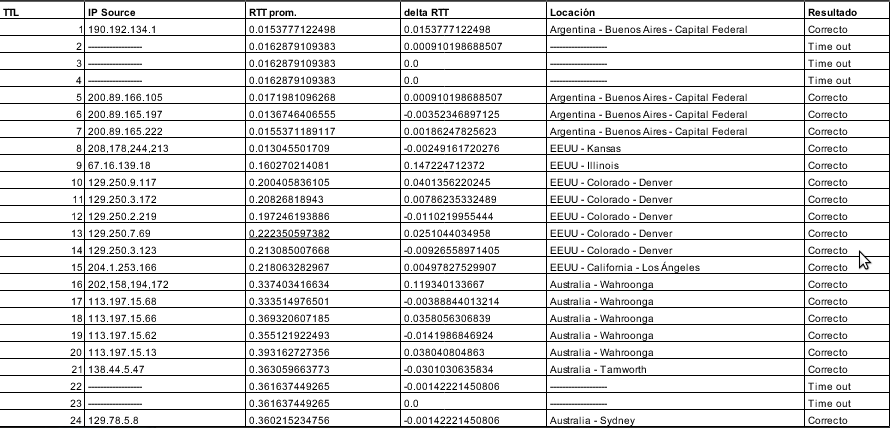
\includegraphics[width=1\textwidth]{img_analisis2/tabla.png} 
	\end{center} 
\end{figure}
%TTL:  1    IP Source: 190.192.134.1    Argentina - Buenos Aires - Capital Federal\\ 
%TTL:  2    Obtuvimos time out, dado que el nodo 2 no contesto. \\
%TTL:  3    Obtuvimos time out, dado que el nodo 3 no contesto. \\
%TTL:  4    Obtuvimos time out, dado que el nodo 4 no contesto. \\
%TTL:  5    IP Source: 200.89.166.105   Argentina - Buenos Aires - Capital Federal\\  
%TTL:  6    IP Source: 200.89.165.197   Argentina - Buenos Aires - Capital Federal\\ 
%TTL:  7    IP Source: 200.89.165.222   Argentina - Buenos Aires - Capital Federal\\ 
%TTL:  8    IP Source: 208.178.244.213  EEUU - Kansas\\ 
%TTL:  9    IP Source: 67.16.139.18     EEUU - Illinois\\ 
%TTL: 10    IP Source: 129.250.9.117    EEUU - Colorado - Denver\\ 
%TTL: 11    IP Source: 129.250.3.172    EEUU - Colorado - Denver\\  
%TTL: 12    IP Source: 129.250.2.219    EEUU - Colorado - Denver\\ 
%TTL: 13    IP Source: 129.250.7.69     EEUU - Colorado - Denver\\ 
%TTL: 14    IP Source: 129.250.3.123    EEUU - Colorado - Denver\\  
%TTL: 15    IP Source: 204.1.253.166    EEUU - California - Los \'Angeles\\
%TTL: 16    IP Source: 202.158.194.172  Australia - Wahroonga\\ 
%TTL: 17    IP Source: 113.197.15.68    Australia - Wahroonga\\ 
%TTL: 18    IP Source: 113.197.15.66    Australia - Wahroonga\\  
%TTL: 19    IP Source: 113.197.15.62    Australia - Wahroonga\\  
%TTL: 20    IP Source: 113.197.15.13    Australia - Wahroonga\\  
%TTL: 21    IP Source: 138.44.5.47      Australia - Tamworth\\ 
%TTL: 22    Obtuvimos time out, dado que el nodo 22 no contesto. \\ 
%TTL: 23    Obtuvimos time out, dado que el nodo 23 no contesto. \\
%TTL: 24    IP Source: 129.78.5.8       Australia - Sydney\newline


De la muestra obtuvimos una distribuci\'on Normal, y los siguientes enlaces submarinos seg\'un el test de Grubbs: al pasar al nodo 9 y al pasar al nodo 16.

\newpage

\subsubsection{An\'alisis de los resultados}
Mediante gr\'aficos haremos un an\'alisis de los resultados obtenidos. \newline


\begin{figure}[h]
	\begin{center}
    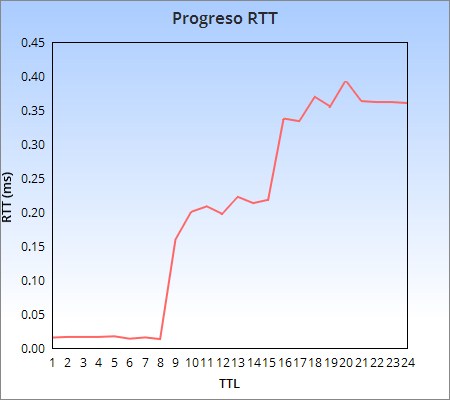
\includegraphics[width=0.5\textwidth]{img_analisis2/RTTprom.png} 
	\caption{Figura 1: Rtt promedio - Universidad de Sydney}	
	\end{center} 
\end{figure}
\vspace{0.25cm}

\begin{figure}[h]
	\begin{center}
    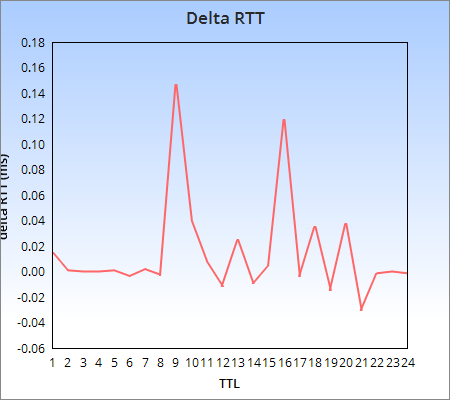
\includegraphics[width=0.5\textwidth]{img_analisis2/Delta_RTT.png}
     \caption{Figura 2: Delta RTT - Universidad de Sydney} 
	\end{center} 
\end{figure}
\vspace{0.25cm}


Podemos ver claramente en los gr\'aficos como en los saltos 9 y 16, que hab\'ian dado como outliers en el test de Grubbs, se denota un cambio brusco tanto en los RTT promedio como en los delta RTT. Con respecto al gr\'afico de RTT promedio podemos ver como de golpe en el salto 9, por ejemplo, sube de 0.013 a 0.15 mili segundos. Mientras tanto, en el gr\'afico de delta RTT, tambi\'en vemos un pico en los saltos marcados como outliers. En este caso se ven aun m\'as claro los outliers ya que se forman picos abruptos.\\
Como la ruta que hacen los paquetes es Argentina-EEUU-Australia, entonces deber\'iamos tener 2 grandes saltos en la traza: Desde Argentina a Estados Unidos (aunque no fuera un enlace submarino s\'i es considerable la distancia (9000 km)), y desde Estados Unidos hasta Australia (en este caso si es un enlace submarino). \newline

Viendo la locallizaci\'on de las ip y los saltos donde nos da el primer outlier, podemos notar que el hop que va desde la  ip 8 (208.178.244.213  EEUU - Kansas) hasta la ip 9 (67.16.139.18     EEUU - Illinois) en realidad no se mueve de Estados Unidos. Creemos que, en realidad, la ip correspondiente al salto n\'umero 8 se encuentra en Argentina pues los RTT de los saltos anteriores (5, 6 y 7), podemos suponer de que el router en realidad est\'a ubicado en alguna parte de Argentina o Sudam\'erica. Creemos que esto sucede porque es un router que brinda servicio a Estados Unidos pero en realidad est\'a f\'isicamente ubicado en Argentina o Sudam\'erica.  \newline

Con respecto al segundo outlier podemos decir que en esta ocaci\'on si se cumple nuestra hip\'otesis. Podemos ver que la ip 15 (204.1.253.166    EEUU - California - Los \'Angeles) se encuetra en el continente americano mientras que la ip 16 (202.158.194.172  Australia - Wahroonga) ya se encuentra en tierras oce\'anicas. \newline

Finalmente presentamos un mapa global donde vamos a trazar los puntos importantes de la ruta que realizan los paquetes. 

\begin{figure}[h]
    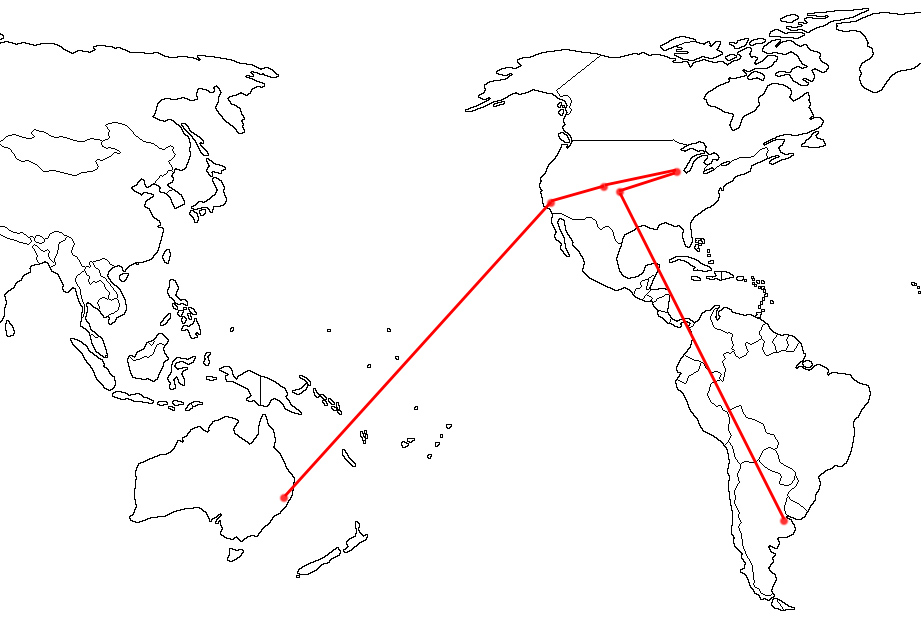
\includegraphics[width=0.7\textwidth]{img_analisis2/mapa-analisis2.jpg}
\end{figure}
\vspace{0.25cm}
